\documentclass{./../div_teaching_slides}

\begin{document}
\title{ECON 340 \\ Economic Research Methods}
\author{Div Bhagia}
\date{Lecture 10: Normal Distribution and Z-Score}

\begin{frame}[noframenumbering, plain]
\maketitle
\end{frame}


%%%%%%%%%%%% 
\begin{frame}{Random Variables}
\begin{witemize}
  \item \textit{Random variables} take different values under different scenarios.
  \item Examples:  outcome from a coin toss or a die roll, or number of times your wireless network fails before a deadline, etc.
  \item The likelihood of these scenarios is summarized by the probability distribution.
  \item Random variables can be \textit{discrete} or \textit{continuous}
\end{witemize}
\end{frame}

%%%%%%%%%%%% 
\begin{frame}{Distribution of a Random Variable}
\begin{witemize}
  \item For a discrete random variable, probability distribution given by the probability of each outcome.
  \item Continuous random variables summarized by the \textit{probability density function}, where area under the curve gives us the probability of an outcome being in an interval. 
 \end{witemize}
\end{frame}

%%%%%%%%%%%% 
\begin{frame}{Probability Density Function}
The area under the curve tells us the probability of an outcome being in a particular interval. \\~\\
\centering
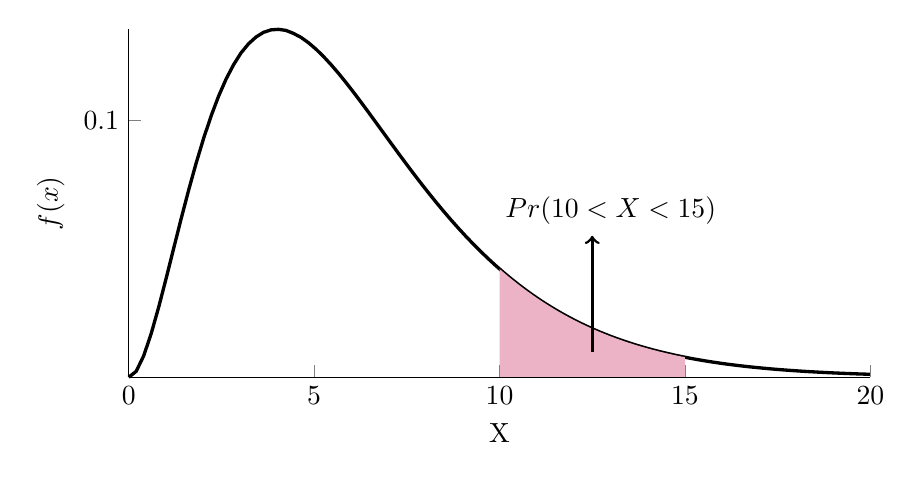
\begin{tikzpicture}[
    declare function={gamma(\z)=
    2.506628274631*sqrt(1/\z)+ 0.20888568*(1/\z)^(1.5)+ 0.00870357*(1/\z)^(2.5)- (174.2106599*(1/\z)^(3.5))/25920- (715.6423511*(1/\z)^(4.5))/1244160)*exp((-ln(1/\z)-1)*\z;},
    declare function={gammapdf(\x,\k,\theta) = 1/(\theta^\k)*1/(gamma(\k))*\x^(\k-1)*exp(-\x/\theta);}
]
\begin{axis}[
  no markers, domain=0:20, samples=100,
  axis lines*=left, xlabel=X, ylabel=$f(x)$,
  %every axis y label/.style={at=(current axis.above origin),anchor=south},
  height=6cm, width=11cm,
  xtick={0,5,10,15,20}, ytick={0.1},
  enlargelimits=false, clip=false, axis on top,
  ]
\addplot [very thick,black] {gammapdf(x,3,2)};
\addplot [fill=purple!30, draw=none, domain=10:15] {gammapdf(x,3,2)} \closedcycle;;
\draw[->, line width=1pt](axis cs: 12.5, 0.01)--(axis cs: 12.5, 0.055);
\node at (axis cs: 13, 0.065) {$Pr(10 <X<15)$};
\end{axis}
\end{tikzpicture}\end{frame}

%%%%%%%%%%%% 
\begin{frame}{Normal Distribution}
One distribution appears more than others --- Normal Distribution \\~\\
\begin{columns}[c]
\begin{column}{0.5\textwidth}
\centering
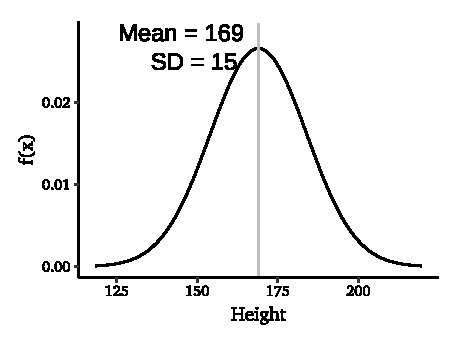
\includegraphics[scale=0.85]{./../../Output/height_norm_pdf.pdf} \\
$ height \sim N(169, 225) $
\end{column}
\begin{column}{0.6\textwidth}
\vspace{-1.5cm}

%%%%%%%%%%%%
What's special about it? \\
\begin{witemize}
\item Symmetric (no skew, mean=median, bell-shaped)
\item Height, birthweight, SAT scores, etc., normally distributed 
\item Sampling distribution approximately normal
\end{witemize}
\end{column}
\end{columns}
\end{frame}

%%%%%%%%%%%%
\begin{frame}{Normal Distribution}
\begin{witemize}
  \item Normal distribution with mean $\mu$ and variance $\sigma^2$ is expressed as $N(\mu,\sigma^2) $
  \item So if I write $X \sim N(12,4) $, it means $X$ is normally distributed with mean 12 and variance 4
  \item The standard normal distribution is the normal distribution with mean 0 and variance 1, denoted by $N(0,1)$
  \item Random variables that have a $N(0,1)$ distribution are often denoted by $Z$
\end{witemize}
\end{frame}

%%%%%%%%%%%% 
\begin{frame}{Normal Distribution}
\centering
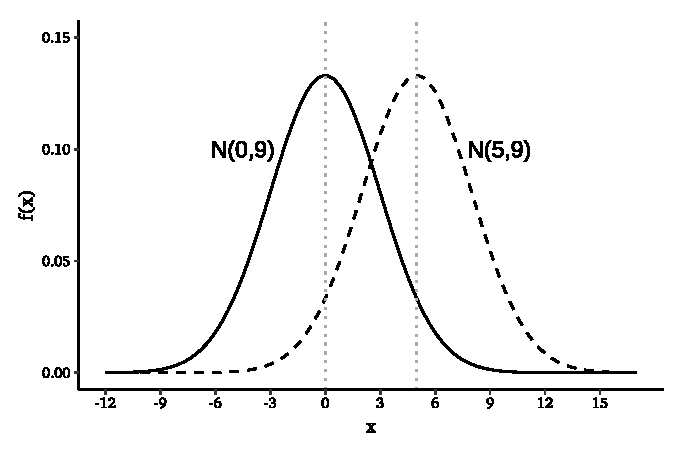
\includegraphics{./../../output/norm1}
\end{frame}


%%%%%%%%%%%% 
\begin{frame}{Normal Distribution}
\centering
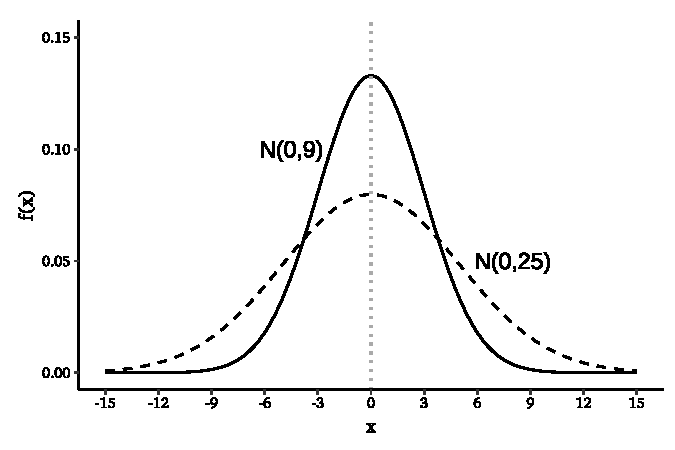
\includegraphics{./../../output/norm2}
\end{frame}

%%%%%%%%%%%%
\begin{frame}{How to find the area under the curve?}
\begin{witemize}
  \item Often interested in finding the probability that a random variable lies in a particular interval
  \item Cumbersome to take the integral each time
  \item Since the normal distribution is so commonly used, one can find these probabilities easily for the \textit{standard normal variable}: $$Z \sim N(0, 1)$$
  \item We can use the standard normal probabilities to get the probabilities for any normally distributed variable
\end{witemize}
\end{frame}

%%%%%%%%%%%%
\begin{frame}{Standardized Random Variables}
A random variable can be transformed into a random variable with mean 0 and variance 1 by subtracting its mean and then dividing by its standard deviation, a process called standardization. \\~\\
$$ Z = \frac{X-\mu_X}{\sigma_X} $$
\end{frame}

%%%%%%%%%%%%
\begin{frame}{How to find the area under the curve?}
For example, say $X \sim N(3, 16)$. We want to calculate $Pr(X \geq 5)$
 \begin{figure}[!h]
 \centering	
\begin{tikzpicture}
\begin{axis}[
  no markers, domain=3-3*4:3+3*4, samples=100,
  axis lines*=left, xlabel=X, ylabel=$f(X)$,
  %every axis y label/.style={at=(current axis.above origin),anchor=south},
  height=6cm, width=10cm,
  xtick={-5, -3, -1, 1, 3, 5, 7, 9, 11}, %ytick=\empty,
  enlargelimits=false, clip=false, axis on top,
  ]
  \addplot [very thick,black] {gauss(3, 4)}; 
  \addplot [fill=purple!20, draw=none, domain=5:3+3*4] {gauss(3, 4)} \closedcycle;
%\draw[->, line width=1pt](axis cs: 185, 0.0125)--(axis cs: 205, 0.0125);
%\node at (axis cs: 0, 0.2) { 95\%};
\end{axis}
\end{tikzpicture}
 \end{figure}
\end{frame}

%%%%%%%%%%%%
\begin{frame}{How to find the area under the curve?}
Given $X \sim N(3, 16)$, 
$$ Z = \frac{X-3}{4} \sim N(0,1) $$

Note that, 
  $$ Pr(X \geq 5) = Pr\left(\frac{\red{X}-3}{4} \geq \frac{\red{5}-3}{4}\right) = Pr(Z \geq 0.5)  $$
 We can now refer to the standard normal table and find that $Pr(Z \geq 0.5)$
\end{frame}

%%%%%%%%%%%%
\begin{frame}{How to find the area under the curve?}
 \begin{figure}[!h]
 \centering	
\begin{tikzpicture}
\begin{axis}[
  no markers, domain=-3:3, samples=100,
  axis lines*=left, xlabel=Z, ylabel=$f(Z)$,
  %every axis y label/.style={at=(current axis.above origin),anchor=south},
  height=6cm, width=10cm,
  xtick={-1.96, 0, 0.5, 1.96}, %ytick=\empty,
  enlargelimits=false, clip=false, axis on top,
  ]
  \addplot [very thick,black] {gauss(0, 1)}; 
  \addplot [fill=purple!20, draw=none, domain=0.5:3] {gauss(0, 1)} \closedcycle;
\node at (axis cs: 1.1, 0.1) {$0.3085$};
\end{axis}
\end{tikzpicture}
 \end{figure}
\end{frame}

%%%%%%%%%%%%
\begin{frame}{Recipe}
Given $X \sim N(\mu, \sigma^2)$, general recipe to find $Pr(x_0<X<x_1)$: \\~\\
\begin{witemize}
  \item Find $z_0 = (x_0-\mu)/\sigma$ and $z_1 = (x_1-\mu)/\sigma$
  \item Use standard normal table to find $Pr(z_0<Z<z_1)$ \\~\\
\end{witemize}

\textit{Example}. Given $X \sim N(3, 16)$, find $Pr(2 < X < 5)$.
\end{frame}

%%%%%%%%%%%%%%%%%%%%
\begin{frame}{Area under the curve}
\begin{witemize}
  \item Alternatively, sometimes we are given $ Pr(X<x)$ or $Pr(X>x)$ and we need to find $x$. 
  \item \textit{Example}: Given $X \sim N(3, 16)$ and $ Pr(X>x) = 0.10$, find $x$. 
  \item Start by finding $z$, such that $Pr(Z>z)=0.1$. From the standard normal table, $z=1.28$.
  \item Now we just need to convert $z$ to $x$.
  \item Since $Z = \frac{X-\mu}{\sigma} \rightarrow X = \mu + Z.\sigma$, so $x = 3+1.28 \times 4 = 8.12$
\end{witemize}
\end{frame}

\end{document}